\subsection{Experimental Results and Findings}


{We report our findings based on a rigorous evaluation across $70$ randomly generated inventory scenarios. To ensure a standardized comparison, we evaluate performance based on expected cost minimization ($\mathds{E}\big[\mathrm{Cost}(\pi)\big]$), assuming a risk-neutral decision-maker (i.e. $\lambda = 10$ in \cref{eqn:objective}).}

{
\Cref{tab:cost_reduction_detailed} summarizes the comparative performance. The results provide strong empirical support for our architectural thesis: separating semantic understanding from logical optimization significantly outperforms end-to-end LLM reasoning.}

\begin{table}[!ht]
    \centering
    \small
    \begin{tabular}{l c c c}
        \toprule
        \textbf{Benchmark \& Scenario} & \textbf{Count ($n$)} & \textbf{\makecell{Avg. Cost Red.\\(Mean \& Std. Dev.)}} & \textbf{\makecell{Win Rate\\(\%)}} \\
        \midrule
        \multicolumn{4}{l}{\textit{\textbf{Baseline 1: vs. GPT-4o (Interactive)}}} \\
        \hspace{1em}Overall Performance & 70 & \textbf{32.1\%} $\pm$ 17.8\% & 97.1\% \\
        \addlinespace[0.5em]
        \hspace{1em}\textit{By Demand Distribution (Lead Time = 7 days)} & & & \\
        \hspace{2em}Normal Distribution & 14 & 34.2\% $\pm$ 15.0\%& 100\% \\
        \hspace{2em}Poisson Distribution & 11 & 33.8\% $\pm$ 19.7\%& 100\%\\
        \addlinespace[0.5em]
        \hspace{1em}\textit{By Lead Time (Demand = Poisson)} & & & \\
        \hspace{2em}Short Lead Time (1 day)  & 15 & 26.8\% $\pm$16.4\% & 93.3\% \\
        \hspace{2em}Long Lead Time (7 days) & 11 & 33.8\% $\pm$19.7\% & 100\% \\
        \midrule
        \multicolumn{4}{l}{\textit{\textbf{Baseline 2: vs. GPT-4o (Parameter Input)}}} \\
        \hspace{1em}Overall Performance & 70 & \textbf{33.4\%} $\pm$ 16.8\% & 100\% \\
        \bottomrule
    \end{tabular}
    \caption{\textbf{Performance Statistics of Hybrid Agentic Framework.} \\
    This table reports the cost reduction statistics (Mean and Standard Deviation) and \\ the win rate (percentage of instances where the Hybrid Agent outperformed the benchmark).}
    \label{tab:cost_reduction_detailed}
\end{table}


To contextualize the economic scale of these experiments, our simulation parameters mirror the operating realities of Small and Medium-sized Enterprises (SMEs). The holding cost in our testbed ranges from \$0.25 to \$4.00 per unit/period, with penalty costs for stockouts ranging significantly higher (averaging roughly \$5.00). Over a standard planning horizon of a few months, the cumulative cost for a single item typically runs into the thousands of dollars. While these unit economics may appear modest in isolation, they scale linearly across the hundreds of SKUs typical of a retail inventory. Consequently, a persistent efficiency gap of roughly 30\% translates into substantial margin erosion for a real-world business, validating the material significance of our findings.



{In the following subsections, we unpack the sources of this advantage in three steps. First, we quantify the aggregate efficiency gap—the ``Hallucination Tax''—in interactive settings (\Cref{sec:hallucination_tax}). Second, we identify the operational conditions that make the agent most valuable (\Cref{sec:driver}). Finally, we isolate the root cause of the baseline's failure by distinguishing between errors of understanding (bad inputs) and errors of reasoning (bad logic) (\Cref{sec:cognitive_ceiling}).}



\subsubsection{The Hallucination Tax (\emph{Treatment A} vs. \emph{B}).}
\label{sec:hallucination_tax}



Our comparison begins with the aggregate performance gap between our Hybrid Agentic Framework (\emph{Treatment A}) and the \emph{GPT-4o} Interactive baseline (\emph{Treatment B}). As detailed in \Cref{tab:cost_reduction_detailed}, the hybrid approach yields a substantial $\mathbf{32.1\%}$ cost reduction (standard deviation $17.8\%$) and achieves a $97.1\%$ win rate across the $70$ test instances. In the rare exceptions ($2$ instances) where \emph{Treatment~B} performs better, the margins are negligible ($2\%$ and $6\%$, respectively), and in both cases, the baseline happens to converge to an $(s, S)$ heuristic effectively identical to the one identified by our optimizer.

We term this efficiency loss the \textbf{``Hallucination Tax.''} It represents the compound penalty incurred when a firm relies on a general-purpose language model as an end-to-end solver. This gap is not merely a reflection of random error, but a structural divergence in how the two systems approach problem-solving: one relies on probabilistic token generation, the other on rigorous mathematical optimization.

\vspace{.5em}

\paragraph{The Fluency Trap: Why Managers Get Fooled.}
A qualitative analysis of the conversation logs reveals a dangerous phenomenon we call the \emph{fluency trap}. The \emph{GPT-4o} baseline is highly eloquent; it correctly uses domain terminology and offers structurally plausible advice. However, this linguistic competence masks a fundamental inability to calibrate policy parameters to specific constraints.

A representative example is observed in the dialogue in \Cref{fig:example1_part2}. Despite explicitly acknowledging a maximum inventory capacity of $80$ units, the \emph{GPT-4o} model confidently recommends: \emph{``When your total inventory... drops to or below 89 units, place an order to bring the inventory up to 80 units.''} 
This recommendation is not merely suboptimal; it is physically impossible. 

For a manager, the model's confident tone creates a false sense of security. The ``Hallucination Tax'' quantifies the cost of this illusion: the difference between a decision that \emph{sounds} correct and one that \emph{is} feasible and optimal. For an SME retailer with net margins of $3$--$5\%$, relying on the ``plausible but suboptimal'' advice of a raw LLM could be the difference between profitability and insolvency.






\subsubsection{Drivers of Performance: When is the Agent Most Valuable?}
\label{sec:driver}

To identify the structural conditions where our framework offers the greatest marginal gains over \emph{GPT-4o} (Interactive), we decompose the results along three dimensions. Our analysis reveals that the value of the Hybrid Framework is not uniform; rather, it scales non-linearly with the complexity and economic consequences of the control problem. \vspace{.5em}


\paragraph{Distribution Agnosticism (Robustness against Tail Risk).}
We examine the system's resilience to demand uncertainty by testing across distinct distribution profiles: Normal distributions (representing high-volume, symmetric demand typical of staples) and Poisson distributions (representing low-volume, right-skewed demand typical of erratic or slow-moving items). 
%
When controlling for lead time (7 days), the agent achieves a $34.2\%$ cost reduction on Normal instances and a comparable $33.8\%$ reduction on Poisson instances. The consistency of these results indicates that the gains from our solver-backed approach are largely agnostic to the underlying demand distribution. 

In inventory control, optimal policies are often determined not by the \emph{average} demand, but by the probability of extreme events in the tail. LLMs, relying on linguistic patterns, tend to exhibit ``bias towards the mean,'' often underestimating the risk of stockouts in skewed (Poisson) scenarios or over-buffering in symmetric (Normal) ones. In contrast, our solver-backed approach explicitly integrates over the full probability density function. This allows the system to remain \emph{distribution agnostic}—delivering precise control for both steady staples and volatile long-tail items. \vspace{.5em}


\paragraph{The Value of Temporal Depth (Impact of Lead Time).}
We evaluate the system's performance across varying supply chain latencies: {Short Lead Times} ($L=1$ day, representing rapid replenishment) and {Long Lead Times} ($L=7$ days, representing cross-regional logistics with delayed fulfillment).
%
On Poisson-demand instances, the performance gap widens significantly with latency. The cost reduction starts at $26.8\%$ for short lead times and expands to $33.8\%$ for long lead times. 

This divergence stems from the challenge of managing \emph{pipeline inventory} (orders placed but not yet received). As lead times grow, a significant portion of stock is ``hidden'' in transit. Basic LLMs and simple heuristics tend to suffer from \emph{myopia}: reacting to immediate on-hand levels while ignoring incoming shipments. In contrast, our Optimization Agent explicitly tracks these in-transit orders as part of the system state. The widening gap indicates that while simple heuristics may suffice when replenishment is nearly immediate, they fail to master the complex intertemporal trade-offs required in high-latency supply chains, where our rigorous solver provides a clearer advantage.  \vspace{.5em}



\paragraph{The Complexity Premium (Impact of Economic Stakes and Action Space).}

We further isolate the parameters driving the largest marginal gains by comparing the structural characteristics of the top and bottom quartiles ($25\%$) of performance improvement. As summarized in \Cref{tab:quartile_analysis}, the analysis confirms a \emph{complexity premium}: the agent's comparative advantage is closely tied to the financial stakes and the richness of the action space.

\begin{table}[!ht]
    \centering
    %\small
    \begin{tabular}{l c c c}
        \toprule
        \textbf{Structural Parameter} & \textbf{\makecell{Top Quartile\\(High Gain)}} & \textbf{\makecell{Bottom Quartile\\(Low Gain)}} & \textbf{\makecell{Significance\\($p$-value)}} \\
        \midrule
        \multicolumn{4}{l}{\textit{\textbf{Economic Stakes}}} \\
        \hspace{1em}Holding Cost & \$1.19 & \$0.71 & $< 0.01$ \\
        \hspace{1em}Penalty Cost & \$6.08 & \$3.84 & $< 0.01$ \\
        \addlinespace[0.5em]
        \multicolumn{4}{l}{\textit{\textbf{Action Space Complexity}}} \\
        \hspace{1em}Max Order Limit & 32.2 & 26.4 & $< 0.02$ \\
        \addlinespace[0.5em]
        \multicolumn{4}{l}{\textit{\textbf{Control Variables (Non-Significant)}}} \\
        \hspace{1em}Set-up Cost & \$3.08 & \$3.06 & $\geq 0.05$ \\
        \hspace{1em}Inventory Capacity & 73.3 & 72.2 & $\geq 0.05$ \\
        \bottomrule
    \end{tabular}
    \caption{\textbf{The Complexity Premium: Structural Characteristics of Top vs. Bottom Quartiles.} \\
    This table compares the average parameter values for instances where the Hybrid Agent achieved the highest cost reductions versus the lowest. While economic stakes and action space show significant divergence, other structural constraints (set-up cost, capacity) do not.}
    \label{tab:quartile_analysis}
\end{table}

\begin{itemize}
    \item \emph{High Economic Stakes Amplify the Cost of Error.} 
    The most significant differentiator is the unit cost structure. Instances in the top quartile exhibit holding costs that are roughly $68\%$ higher and penalty costs that are $58\%$ higher than those in the bottom quartile. This indicates that simple heuristics or vanilla LLMs may perform adequately when items are cheap and the ``forgiveness'' for error is high. However, when the trade-off between holding inventory and losing sales is financially consequential, the precision of a formal solver becomes indispensable.
    
    \item \emph{Broader Action Spaces Reward Optimization.} 
    The top quartile is also characterized by a significantly looser maximum order limit ($32.2$ vs. $26.4$). A tighter limit artificially constrains the solution space, forcing all policies—optimal or heuristic—to converge. Conversely, a broader limit expands the decision boundaries. Our Agentic Framework exploits this flexibility to discover sophisticated replenishment strategies, whereas the baseline tends to fall back on conservative, static heuristics that fail to use the full range of valid actions.
\end{itemize}

It is worth noting that other structural constraints, such as set-up cost and inventory capacity, showed no statistically significant divergence. Taken together, these findings suggest that the Hybrid Agentic Framework is especially beneficial in high-cost, high-flexibility settings, where precision in policy optimization matters most and naive heuristics leave substantial value on the table.





\subsubsection{Isolating the Source of Error: The Failure of Perfect Information (\mbox{\emph{Treatment A}} vs. \emph{C}).}
\label{sec:cognitive_ceiling}

Given the significant efficiency loss observed in the interactive setting, a natural question arises: \emph{Is this failure driven by linguistic ambiguity or computational limitation?} One might hypothesize that the LLM underperforms primarily because the messiness of natural language prevents it from extracting the correct problem parameters.
\emph{Treatment C} tests this hypothesis by removing the communicative burden entirely. We feed the ``ground-truth parameter file'' directly to \emph{GPT-4o}, granting it a complete, noise-free view of the inventory environment. If the bottleneck were solely informational, performance should converge toward the optimal benchmark.
\vspace{-1em}

\paragraph{The Persistence of the Heuristic Tax.}The empirical results decisively reject this hypothesis. As shown in \Cref{tab:cost_reduction_detailed}, providing perfect information yields no statistical improvement over the noisy interactive baseline ($p$-value $= 0.66$). The system hits a hard \emph{Cognitive Ceiling}.

Revisiting the representative instance from \Cref{sec:example1} clarifies exactly what improves—and what remains broken—under perfect information:
\begin{itemize}
\item \emph{In Treatment B (Interactive),} the noise of conversation leads to logical incoherence. The model hallucinates a reorder point ($89$) that violates the capacity constraint ($80$). This is an \emph{Interpretive Error}.
\item \emph{In Treatment C (Perfect Info),} this specific hallucination disappears. With clear access to the parameters, the model respects the capacity limit. However, it still recommends a suboptimal policy (e.g., $(40, 65)$) based on a heuristic estimation of the mean, failing to optimize for the tail risk of stockouts.
\end{itemize}
This reveals that while better data can cure logical hallucinations, it cannot cure the fundamental deficit in stochastic reasoning.
\vspace{.5em}

\paragraph{The Indispensability of Operations Research.}This finding brings us to a critical architectural conclusion regarding the role of General Purpose AI. One might argue that future iterations of foundation models will eventually close this gap without the need for external solvers. Our results suggest otherwise.
Relying on a generalist model to perform stochastic optimization is inherently inefficient and unreliable. To replicate the precision of a dedicated OR solver, a Large Language Model must generate extensive chains of thought, consuming vast amounts of tokens and computational resources to approximate what a standard algorithm (e.g., dynamic programming) can solve in milliseconds. Furthermore, probabilistic token generation remains fundamentally prone to stochastic drift—it can produce numbers that \emph{look} plausible but are mathematically groundless.
Therefore, the ``Last Mile'' of decision support cannot be bridged by scaling model size alone. It requires a division of labor: using the LLM for what it does best (semantic interpretation) and the OR solver for what it does best (deterministic optimization). This hybrid architecture is not merely an engineering patch but a necessary epistemological bridge between descriptive language and normative optimality.




\subsection{Qualitative Analysis on a Representative Instance.}\label{sec:example1}

We conclude this section by presenting conversation logs from \emph{Treatments A--C} on a representative instance. Example 1 demonstrates a scenario where the user approaches the system with a broad background description of a bike repair shop. This behavior is typical of the interactions observed in our experiments.


\begin{figure}[!t]
    \centering
    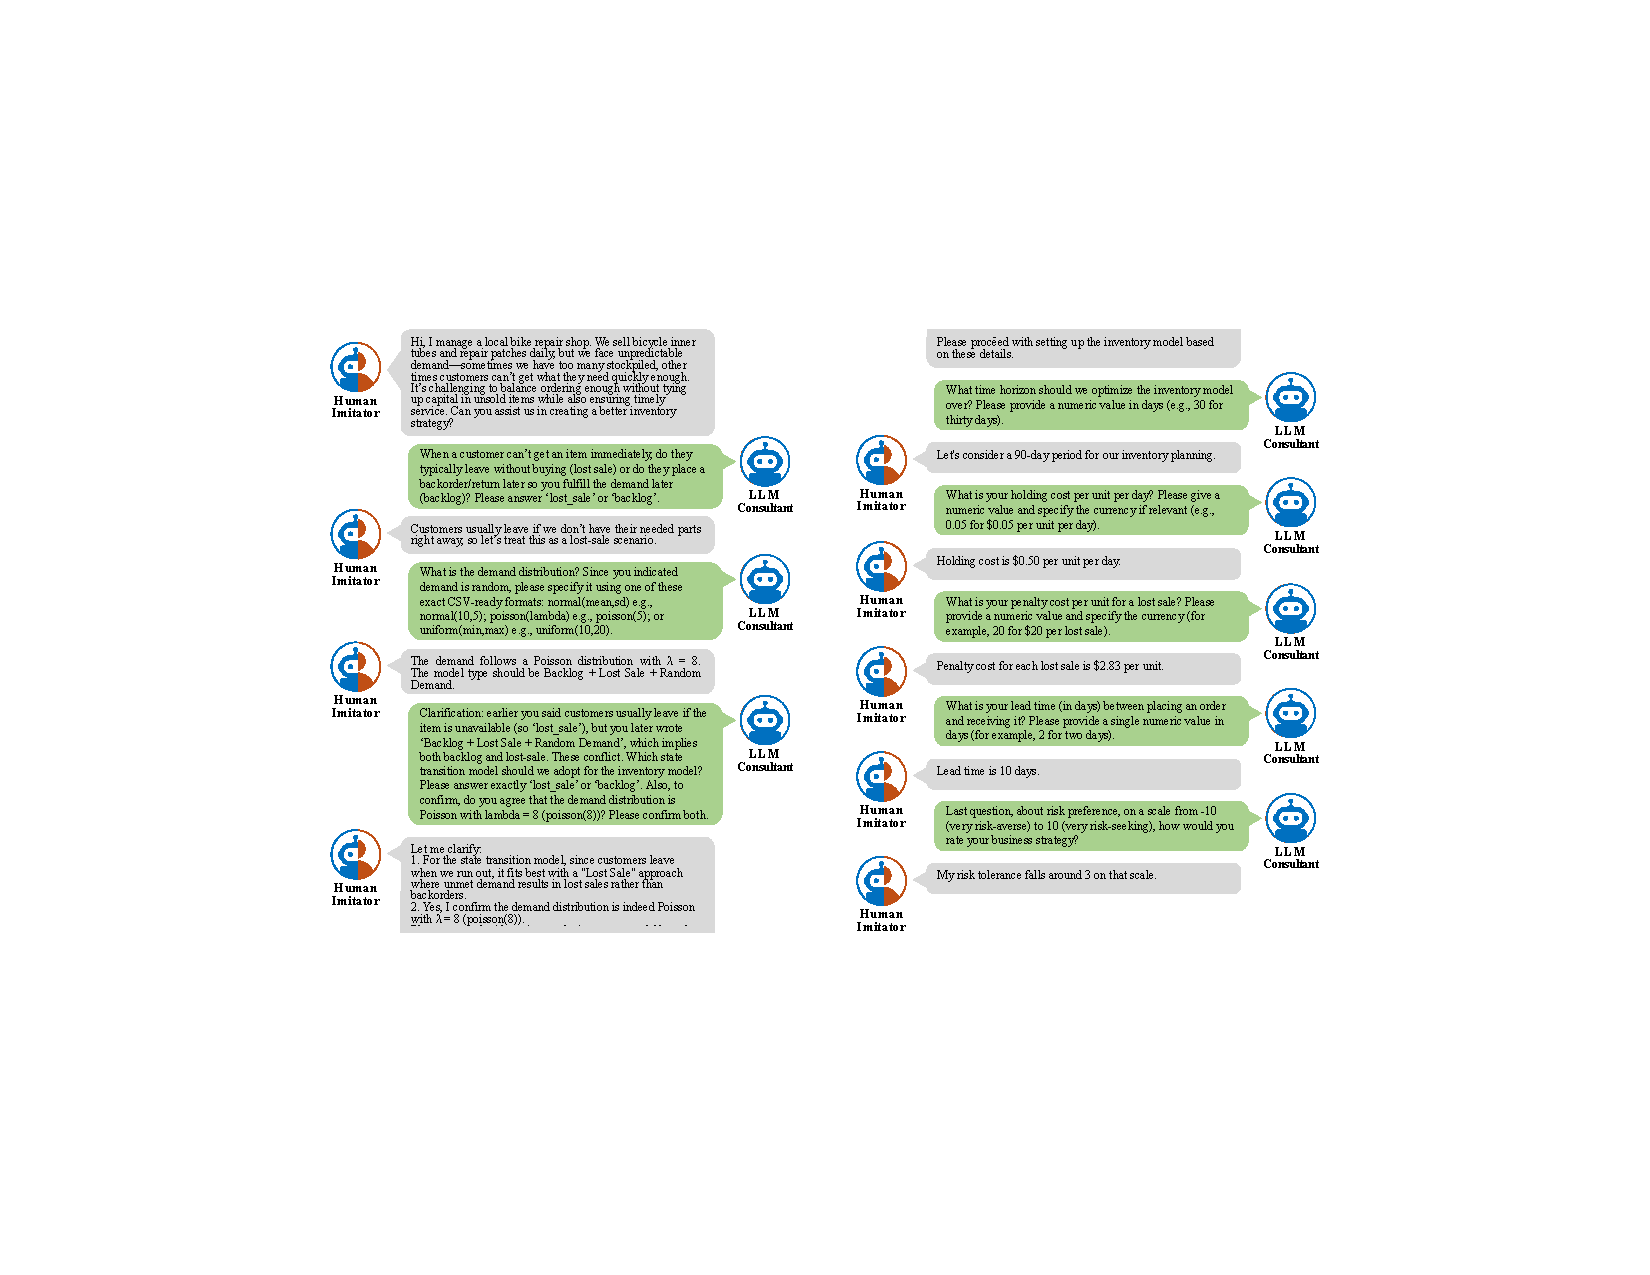
\includegraphics[width=\textwidth, keepaspectratio]{fig/1_Conversation_Log.pdf}
    \caption{\textbf{Example 1 - Treatment A.} Complete conversation logs (Interactive Agent).}
    \label{fig:example1_part1}
\end{figure}


\begin{figure}[!t]
    \centering
    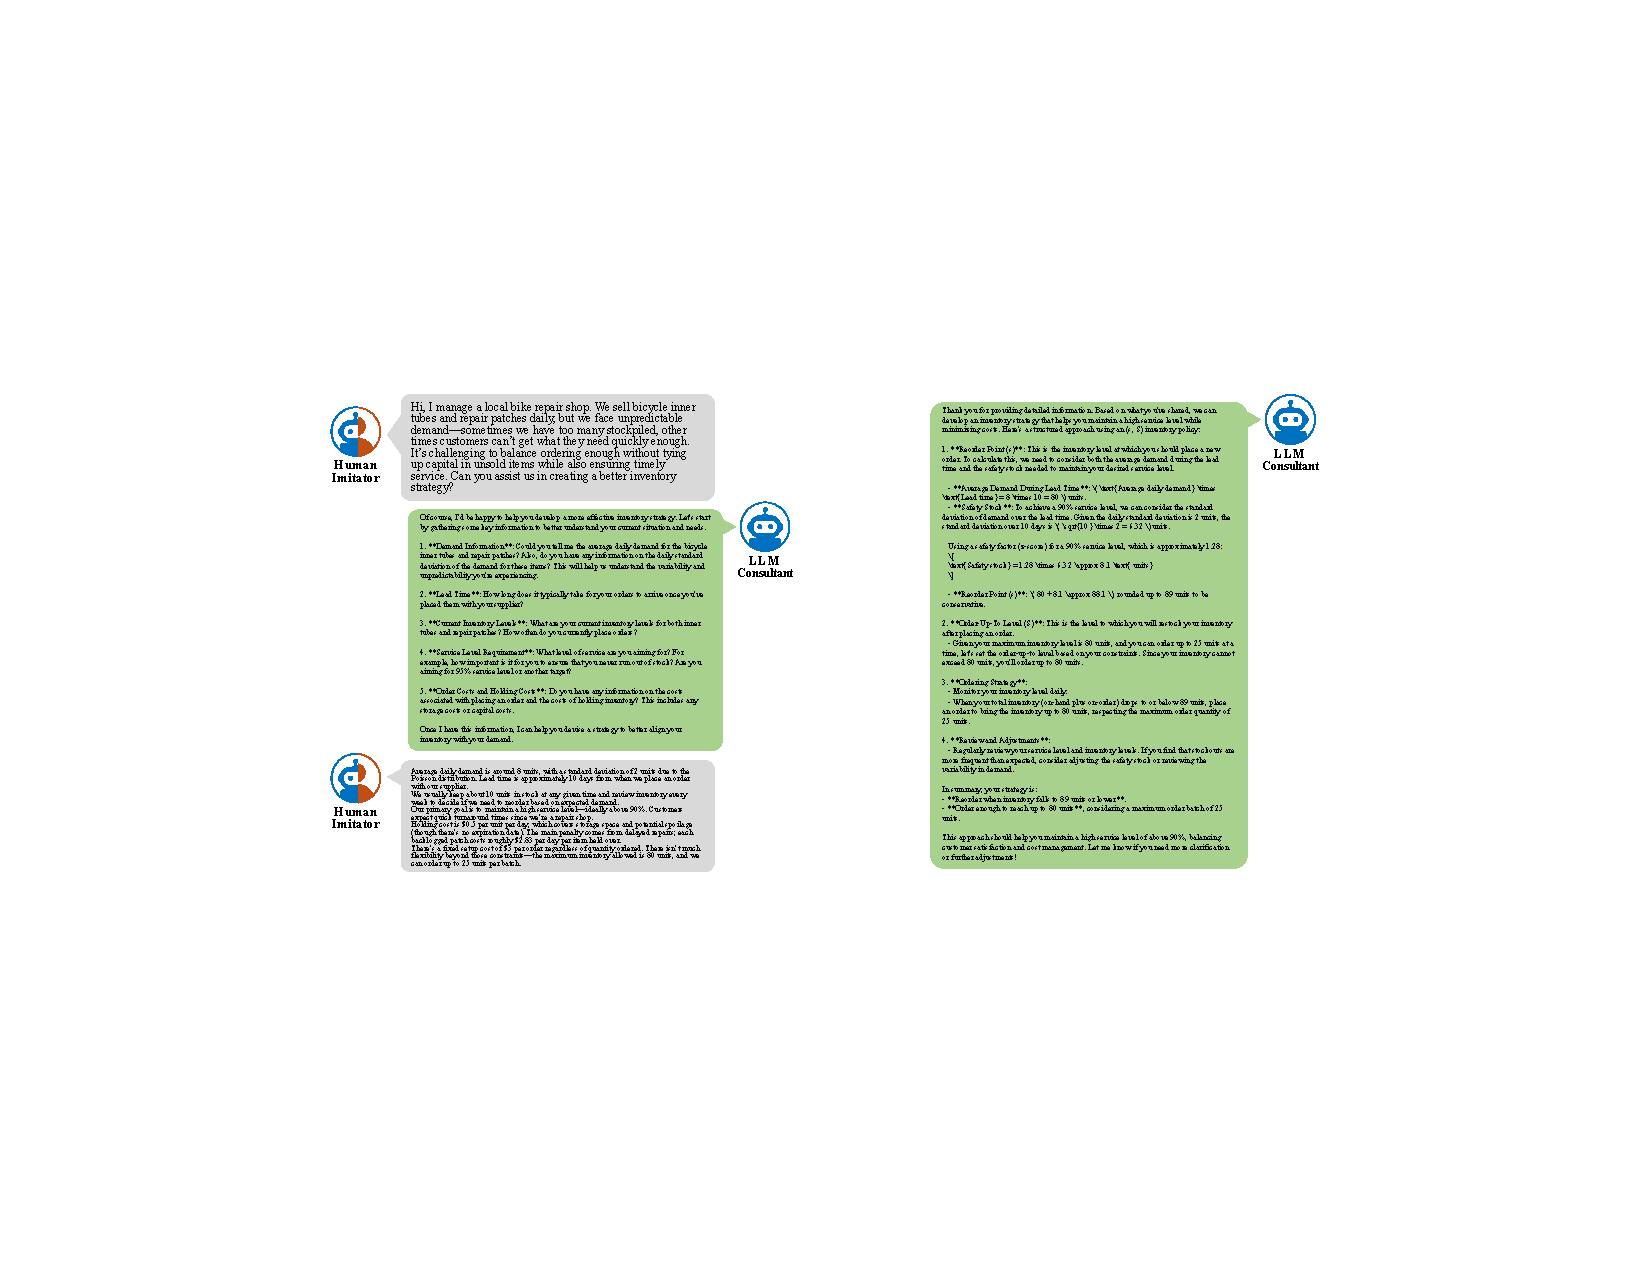
\includegraphics[width=\textwidth, keepaspectratio]{fig/1_GPT_Interaction_Conversation.pdf}
    \caption{\textbf{Example 1 - Treatment B.} Complete conversation logs (GPT-4o Interactive).}
    \label{fig:example1_part2}
\end{figure}


\begin{figure}[!t]
    \centering
    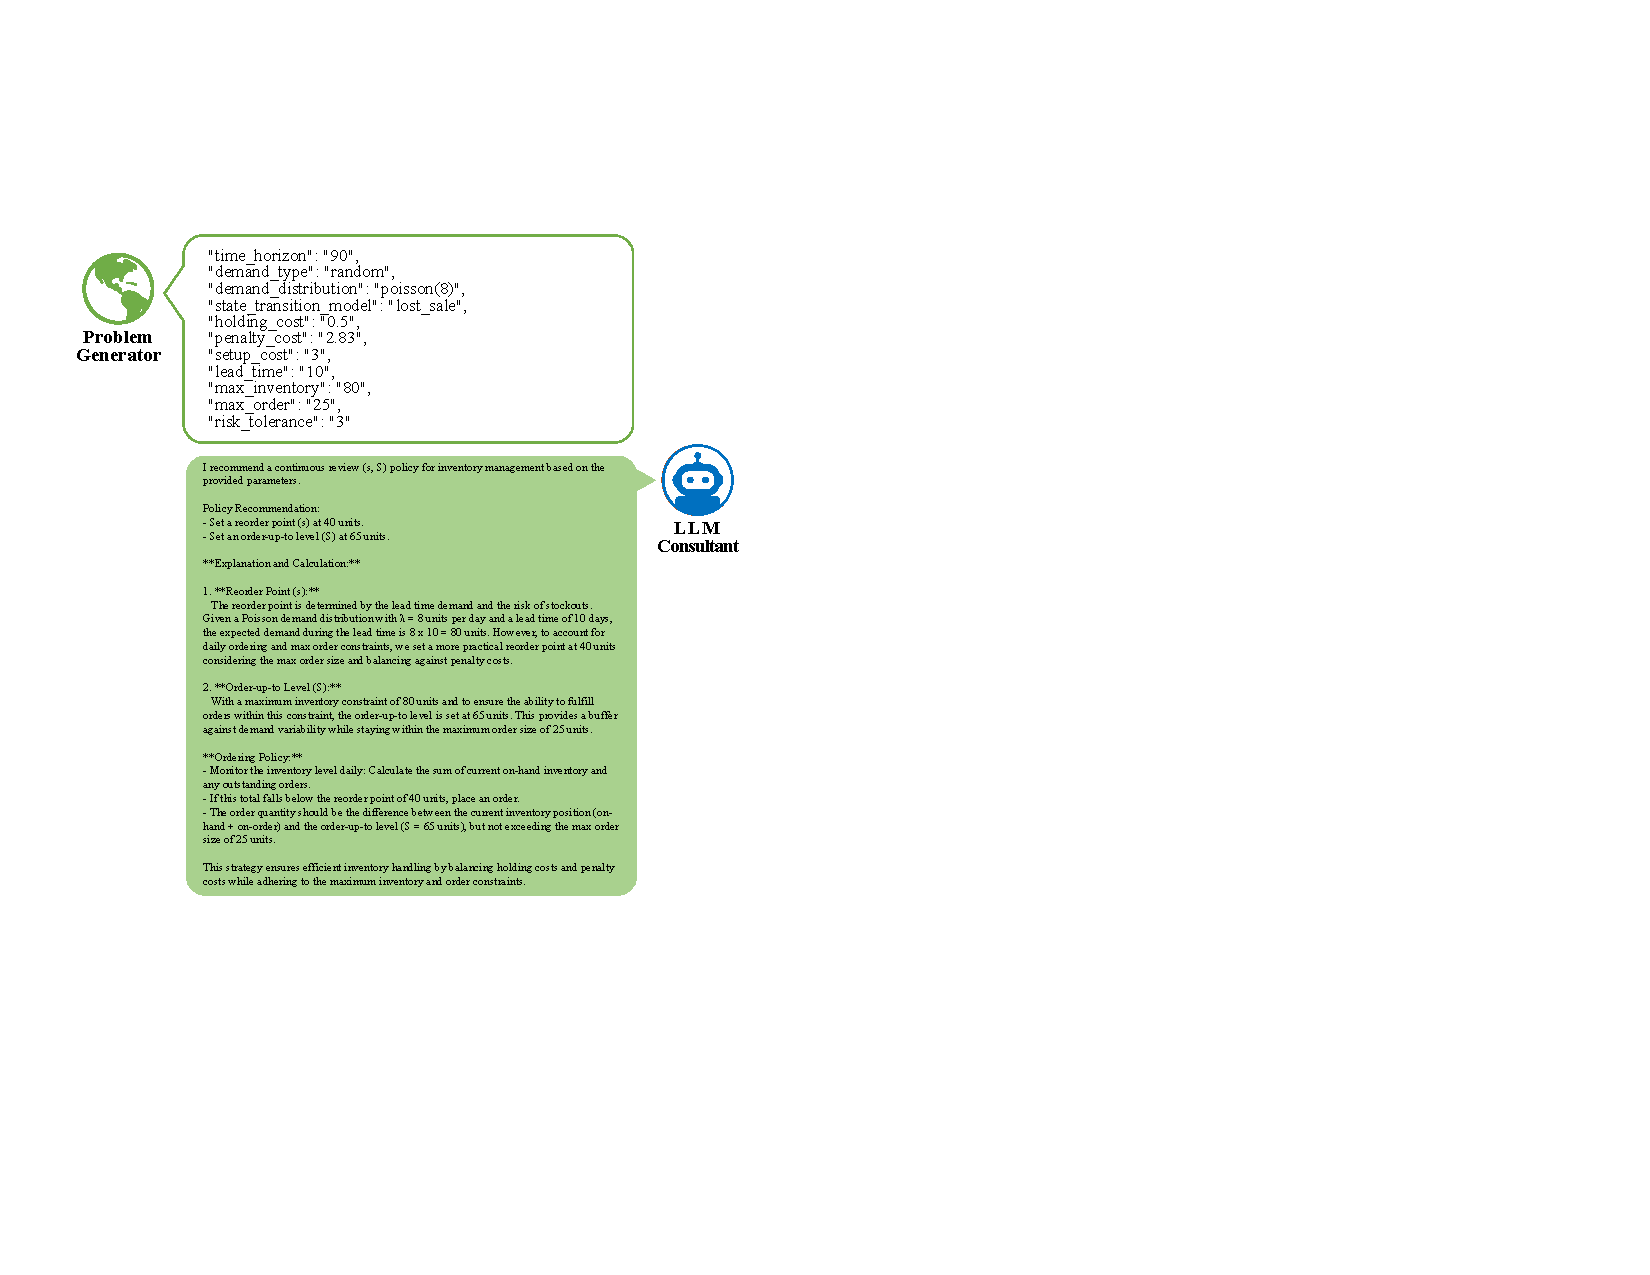
\includegraphics[width=0.7\textwidth, keepaspectratio]{fig/1_GPT_Params.pdf}
    \caption{\textbf{Example 1 - Treatment C.} Complete conversation logs (GPT-4o Parameter Input).}
    \label{fig:example1_full}
\end{figure}

Our \textit{Agentic Framework (Treatment A)} (\Cref{fig:example1_part1}) follows a rigorous slot-filling and verification process. Notably, the agent detects a logical inconsistency when the user initially specifies a ``lost-sale'' model but later requests a ``Backlog + Lost Sale'' model. The agent explicitly flags this conflict (``These conflict'') and prompts the user to select a single valid transition model. After approximately nine rounds of dialogue to resolve such ambiguities and gather all necessary parameters (e.g., time horizon, costs, capacities), the agent forwards a verified parameter set to the Optimization Agent.

In contrast, the \textit{GPT-4o Interactive (Treatment B)} baseline (\Cref{fig:example1_part2}) collects relatively less detailed information, typically asking only for summary statistics (e.g., mean and standard deviation) instead of the full demand distribution required for rigorous modeling. Moreover, it relies on internal heuristics to generate a policy, often leading to hallucinations or feasibility violations. Crucially, in this instance, the baseline recommends an $(s, S)$ policy with a reorder point of 89 units, despite previously acknowledging a maximum inventory capacity of only 80 units. This recommendation is physically impossible to implement. The \textit{GPT-4o Parameter Input (Treatment C)} baseline (\Cref{fig:example1_full}) generates yet another distinct policy ($(s, S)$ with $s=40, S=65$), highlighting the inconsistency and lack of robustness in direct LLM reasoning compared to our solver-backed approach.


Additional conversation logs are provided in \Cref{sec:sample_conversation}. In most instances, the \textit{GPT-4o} baselines rely on simple heuristics to generate standard policies, such as $(s, S)$ or $(R, Q)$. Even in instances where the $(s, S)$ policy structure is preferred, our system applies grid search to mathematically optimize the $s$ and $S$ parameters, whereas \emph{GPT-4o} merely approximates them using basic heuristics.













